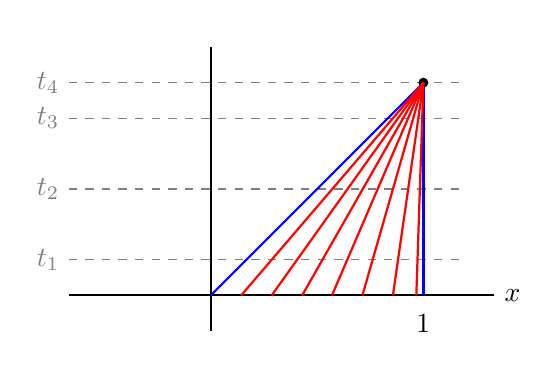
\begin{tikzpicture}[scale=0.9]
%axis
\draw[thick] (-2,0)--(4,0) node[right]{$x$};
\draw[thick] (0,-0.5)--(0,3.5) node[above]{ };

\node[label={below:$1$}] at (3,0) {};

\draw[thick, blue](3,0) -- (3,3);

\draw[thick, blue](0,0) -- (3,3);

\fill (3,3) circle [radius=2pt];

\draw[dashed, opacity=0.5] (3.5, 0.5) -- (-2,0.5) node[left] {$t_1$};
\draw[dashed, opacity=0.5] (3.5, 1.5) -- (-2,1.5) node[left] {$t_2$};
\draw[dashed, opacity=0.5] (3.5, 2.5) -- (-2,2.5) node[left] {$t_3$};
\draw[dashed, opacity=0.5] (3.5, 3) -- (-2,3) node[left] {$t_4$};

% caracteristicas
\draw[thick, red](0.43,0) -- (3,3);
\draw[thick, red](0.86,0) -- (3,3);
\draw[thick, red](1.29,0) -- (3,3);
\draw[thick, red](1.71,0) -- (3,3);
\draw[thick, red](2.14,0) -- (3,3);
\draw[thick, red](2.57,0) -- (3,3);
\draw[thick, red](2.9,0) -- (3,3);

\end{tikzpicture}